\documentclass[tikz]{standalone} % border={left bottom right top}
\input{./Tensors_2.tex}
%!TEX root = thesis.tex
%%%%%%%%%%%%%%%%%%%%%
\def\ri{\mathrm i}
\def\re{\mathrm e}
\def\rd{\mathrm d}
\def\rD{\mathcal D}
\def\hc{{\rm h.c.}}
\def\tr{{\rm tr}}
\def\C{\mathcal{C}}
\def\DC{\Delta\C}
\def\GX{\Gamma X}
\def\DCav{\overline{\Delta\C}}
\def\up{\uparrow}
\def\down{\downarrow}
\def\pdag{{\vphantom\dag}}
\def\pp{\vphantom{n'}}
\def\Cav{\overline\C}
\def\MH{H}
\def\HS{\mathcal{H}}
\def\FS{\mathcal{F}}
\def\omegaT{\tilde{\omega}}
\def\tbc{{\\[1cm]\bf \color{red}[TO BE CONTINUED...]}}
\newcommand{\ave}[1]{\langle #1 \rangle}
\newcommand{\sign}[1]{\text{sign}\left( #1 \right)}
\newcommand{\commutator}[1]{\left[ #1 \right]}
\newcommand{\anticommutator}[1]{\left\{ #1 \right\}}
\newcommand{\brlr}[1]{\left( #1 \right)}
\newcommand{\abs}[1]{\left| #1 \right|}

\usepackage{braket}
\begin{document}

\tikzset{
    %Define standard arrow tip
    >=stealth'
}

\tikzset{
    tst/.style={
      thin, opacity=0.5,
      dashed
    },
    my-arc/.style={
      start angle=0, end angle=360,radius=0.4
    }
  }

\tikzset{
    tst/.style={
      thin, opacity=0.5,
      dashed
    },
    my-arc2/.style={
      start angle=0, end angle=360,radius=0.2
    }
  }

\definecolor{blue}{rgb}{0.2745098039, 0.5333333333, 0.9450980392}
\definecolor{red}{rgb}{0.9176470588, 0.2588235294, 0.2078431373}
\definecolor{yellos}{rgb}{0.9764705882, 0.7333333333, 0.1764705882}
\definecolor{green}{rgb}{0.2039215686, 0.662745098, 0.3176470588}


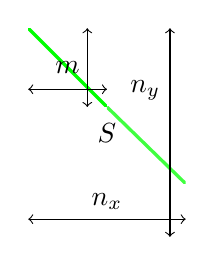
\begin{tikzpicture}
    \rTens{white}{2}{2.65}{(0,0)}
    \rTens{white}{1}{1}{(-.5,.825)}
    \begin{scope}
        \clip (-1,1.325) rectangle (0,0.325);
        \draw[green,very thick](-1,1.325)--(0,0.325);
    \end{scope}
    \begin{scope}
        \clip (0,0.325) rectangle (1,-0.65);
        \draw[green!75!white, very thick](0,0.325)--(1,-.65);
    \end{scope}
    % \node at (-.5,.825) {\color{black}$S$};
    \node at (0,0) {\color{black}$S$};
    % \node[above] at (0,-1.325) {\color{black}$n_x$};
    % \node[left] at (1,0) {\color{black}$n_y$};
    % \node[below] at (-.5,0.33125) {\color{black}$m$};
    % \node[right] at (0,0.825) {\color{black}$m$};

    \draw[black, <->] (-1, -1.1) -- (1, -1.1) node[pos=.5, above] {\color{black}$n_x$};
    \draw[black, <->] (.8, -1.325) -- (.8, 1.325) node[pos=.7, left] {\color{black}$n_y$};

    \draw[black, <->] (-1, 0.55) -- (0, 0.55);
    \draw[black, <->] (-.25, 0.325) -- (-.25, 1.325);

    \node at (-.5,0.825) {$m$};
\end{tikzpicture}


\end{document}
